\section{溶液濃度による高速化への影響}
\label{sec:concentration}
超音波照射された擬塑性流体中を落下する球における高速化に関して,溶液濃度による影響を考えるため,溶液濃度を変化させて実験を行った.実験条件をTable.\ref{table:exp-conditions}に示す.落下球の高速化に関して,式(\ref{eq:Udiff})より球径による影響を受けるが,今回の実験条件において濃度変化による影響よりも十分に小さいものとして,球径は同一であるとして考える.

PAA溶液濃度と終端速度の関係をFig.\ref{fig:concentrationUT}に示す.溶液濃度が濃くなると,終端速度が遅くなった.これは,濃度が濃くなると粘度$\mu$が大きくなり,粘性による抵抗が大きくなるためであると考えられる.式(\ref{eq:UT0})において,濃度が濃くなると$k$が大きく,$n$が小さくなるためである.PAA溶液濃度と高速化度合の関係をFig.\ref{fig:concentrationUdiff}に示す.縦軸は高速化度合$U_\text{on}/U_\text{off}$,横軸はPAA溶液濃度である.アルミニウム,アルミナにおいてはPAA濃度1.0wt.\%が高速化の極大であった.一方でステンレスは明瞭な高速化の極大が見られなかったが,PAA濃度0.7-1.3wt.\%のいずれかに高速化の極大が存在すると考えられる.また,真鍮においてPAA濃度0.7wt.\%が高速化の極大であった.これらより,濃度が濃くなると高速化が顕著になるが,濃すぎると高速化がみられにくくなることが分かった.

式(\ref{eq:UdiffRho})を用いて,落下球の密度,溶液濃度の影響を整理した結果をFig.\ref{fig:concentrationUdiff2}に示す.縦軸は高速化度合$U_\text{on}/U_\text{off}$,横軸は密度変化,濃度変化による影響を考慮した値である.アルミニウムにおいては濃度の上昇に伴い高速化が顕著となる正の相関が見られた.アルミナにおいて,PAA濃度1.0wt.\%で高速化が顕著になり,それ以上の濃度においては高速化がみられにくくなった.ステンレスにおいて,濃度との相関が不明瞭であった.真鍮において,PAA濃度0.7wt.\%の濃度で高速化が顕著になった.これらをまとめた結果をFig.\ref{fig:concentrationUdiffAll}に示す.超音波照射による高速化度合は,密度変化,粘度変化に対して弱い正の相関がみられた.濃度変化による高速化度合への影響は存在するが,別の要因が生じているため弱い正の相関となったと考えられる.本研究\ref{sec:elasticity-discussion}章において,高速化への影響を与えていると考えられる,弾性による影響の議論を行う.

\begin{figure}[ht]
    \centering
    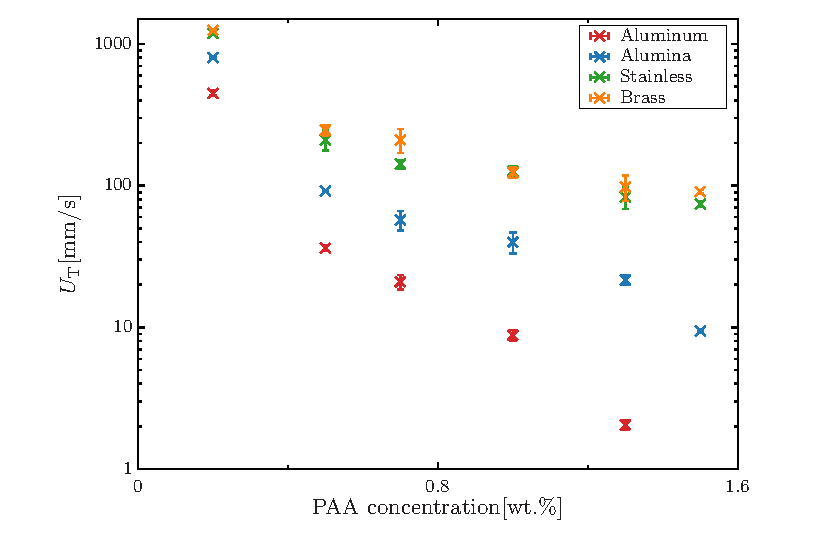
\includegraphics[width=0.8\textwidth]{./5-Results/concentrationUT.eps}
    \caption{Termination velocity in PAA solution concentration.}
    \label{fig:concentrationUT}
\end{figure}

\begin{figure}[ht]
    \centering
    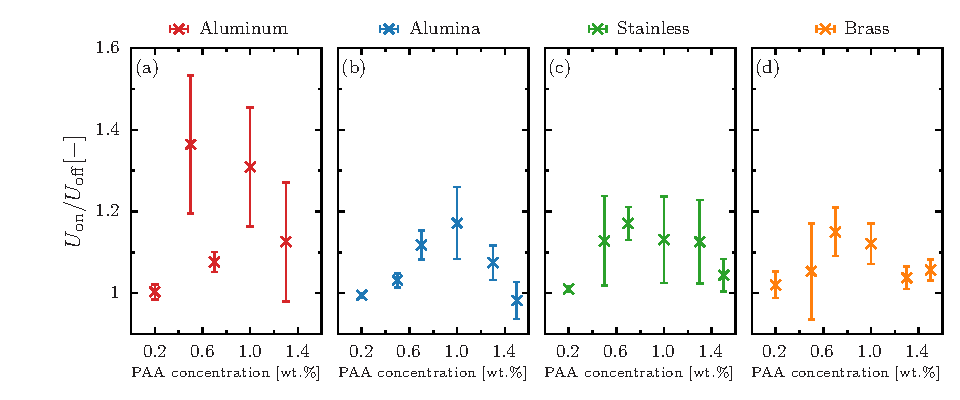
\includegraphics[width=1.0\textwidth]{./5-Results/concentrationUdiff.eps}
    \caption{Velocity ratio in PAA solution concentration (a)Aluminum, (b)Alumina, (c)Stainless, (d)Brass.}
    \label{fig:concentrationUdiff}
\end{figure}

\begin{figure}[ht]
    \centering
    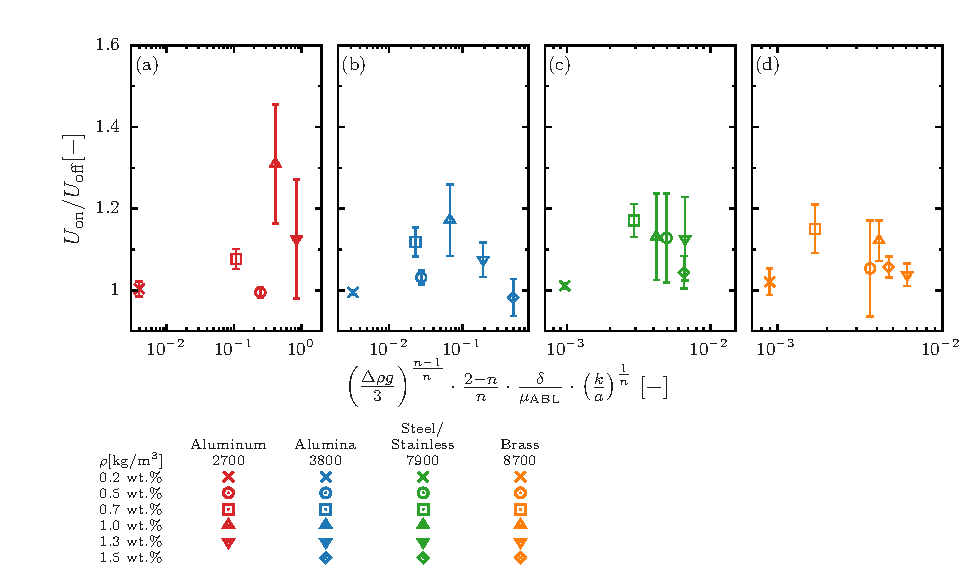
\includegraphics[width=1.0\textwidth]{./5-Results/concentrationUdiff_each.eps}
    \caption{Velocity ratio in PAA solution concentration (a)Aluminum, (b)Alumina, (c)Stainless, (d)Brass.}
    \label{fig:concentrationUdiff2}
\end{figure}

\begin{figure}[ht]
    \centering
    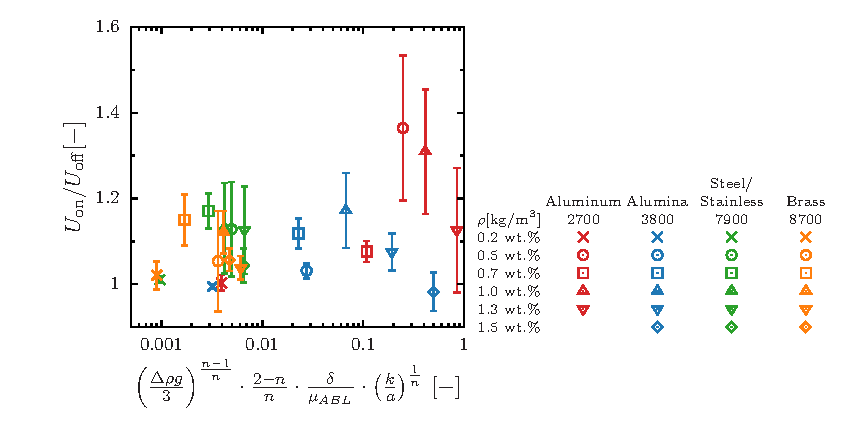
\includegraphics[width=0.7\textwidth]{./5-Results/concentrationUdiffAll.eps}
    \caption{Relationship between density, viscosity and terminal velocity.}
    \label{fig:concentrationUdiffAll}
\end{figure}